
\begin{figure*} 
\begin{subfigure}[t]{0.12\linewidth}
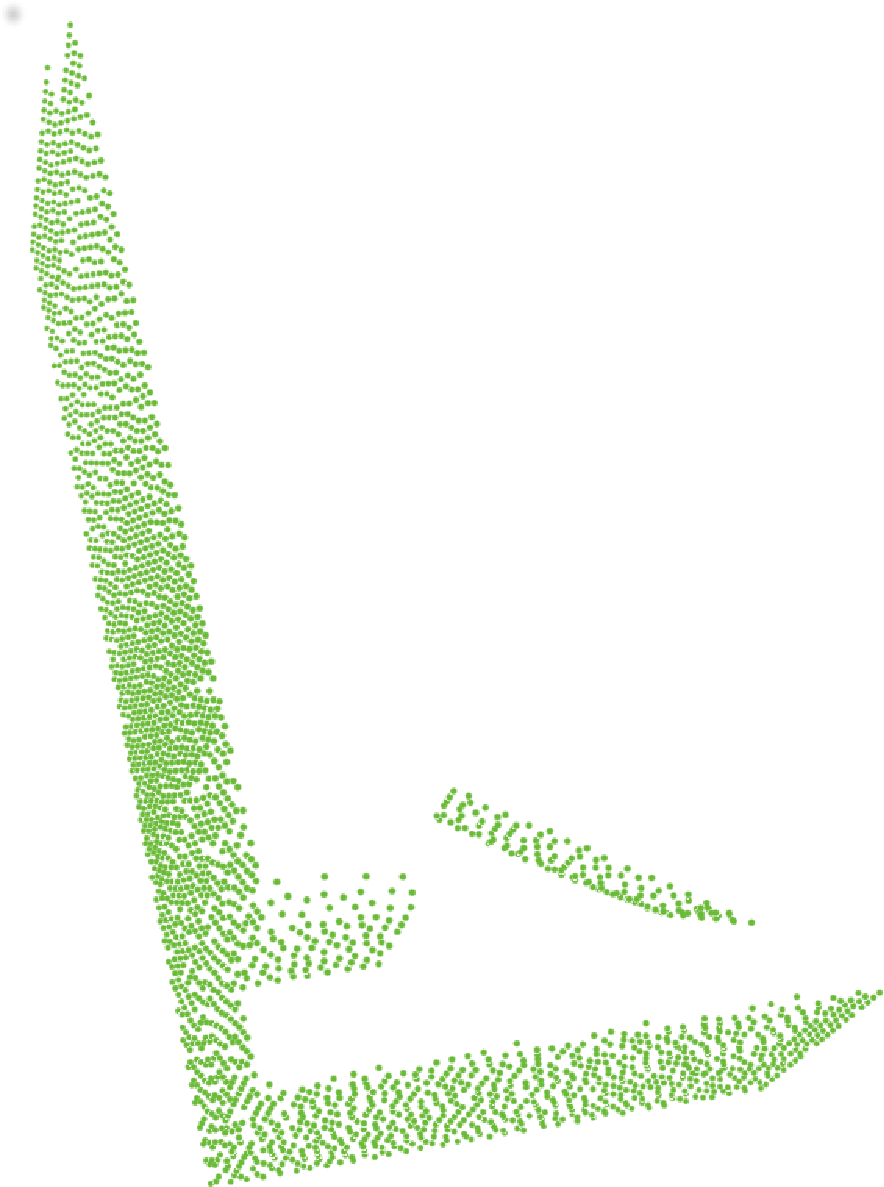
\includegraphics[width=0.8\linewidth]{images/pc-sofa1.pdf}
\end{subfigure}
\hfill
\begin{subfigure}[t]{0.12\linewidth}
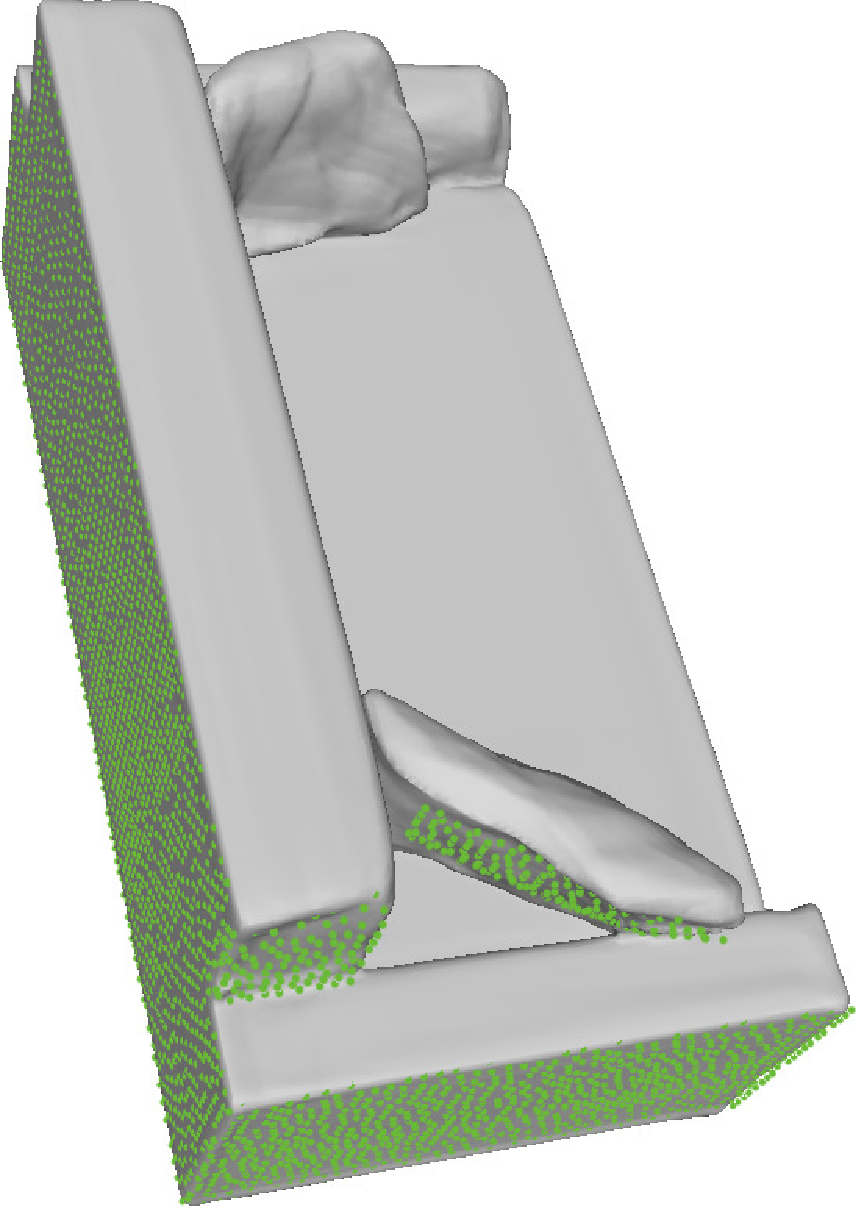
\includegraphics[width=0.8\linewidth]{images/overlay-sofa1.pdf}
\end{subfigure}
\hfill
\begin{subfigure}[t]{0.24\linewidth}
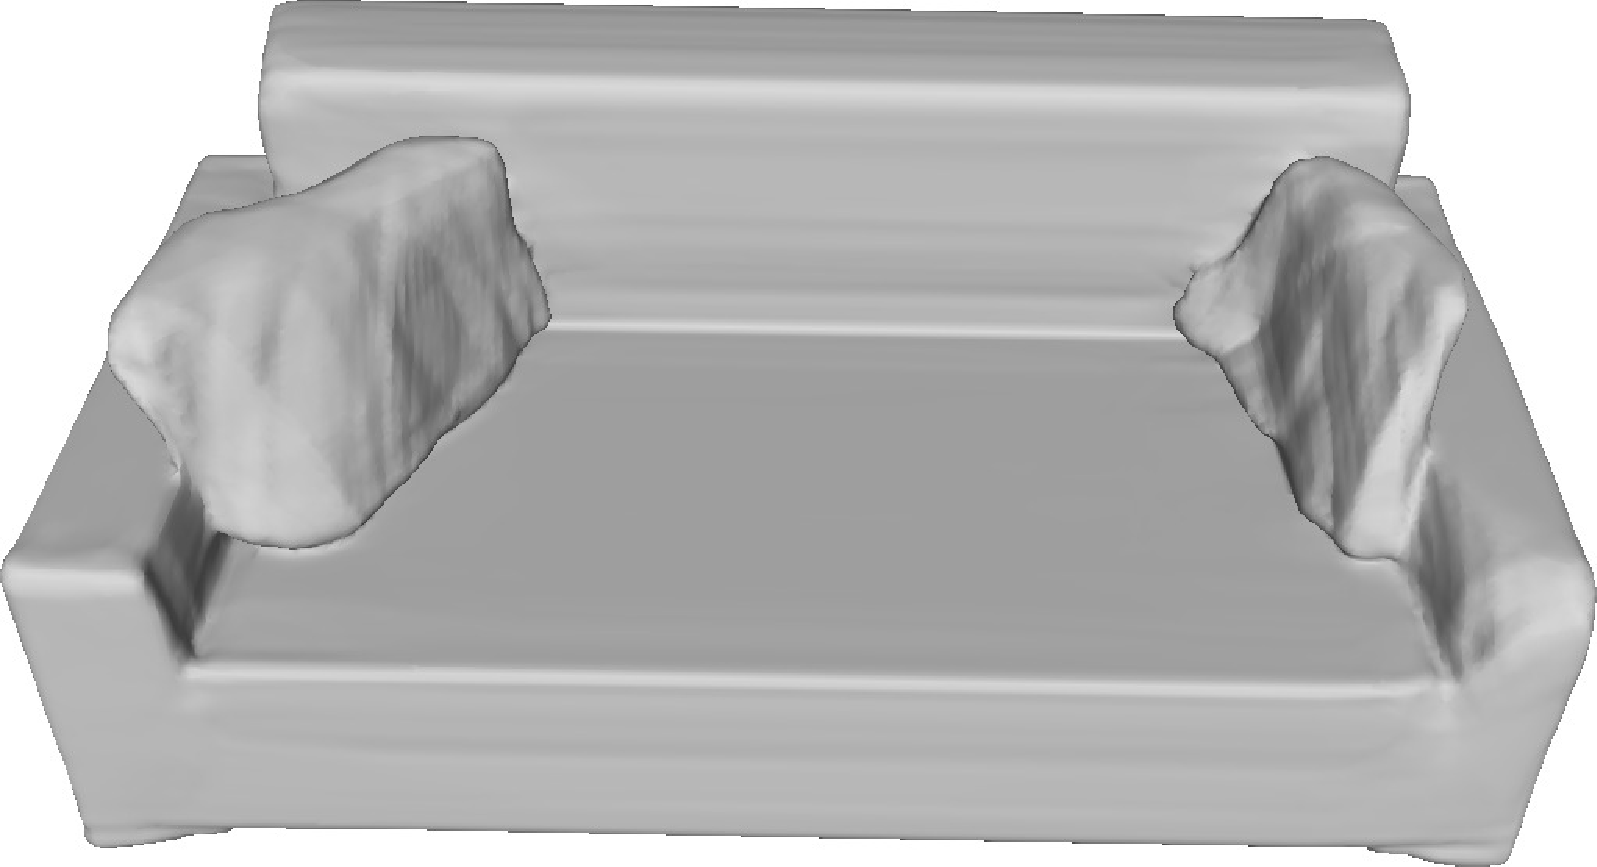
\includegraphics[width=0.8\linewidth]{images/completion-sofa1.pdf}
\end{subfigure}
\begin{subfigure}[t]{0.24\linewidth}

\includegraphics[width=0.8\linewidth]{images/gt-sofa1.pdf}
\end{subfigure}
\begin{subfigure}[t]{0.23\linewidth}
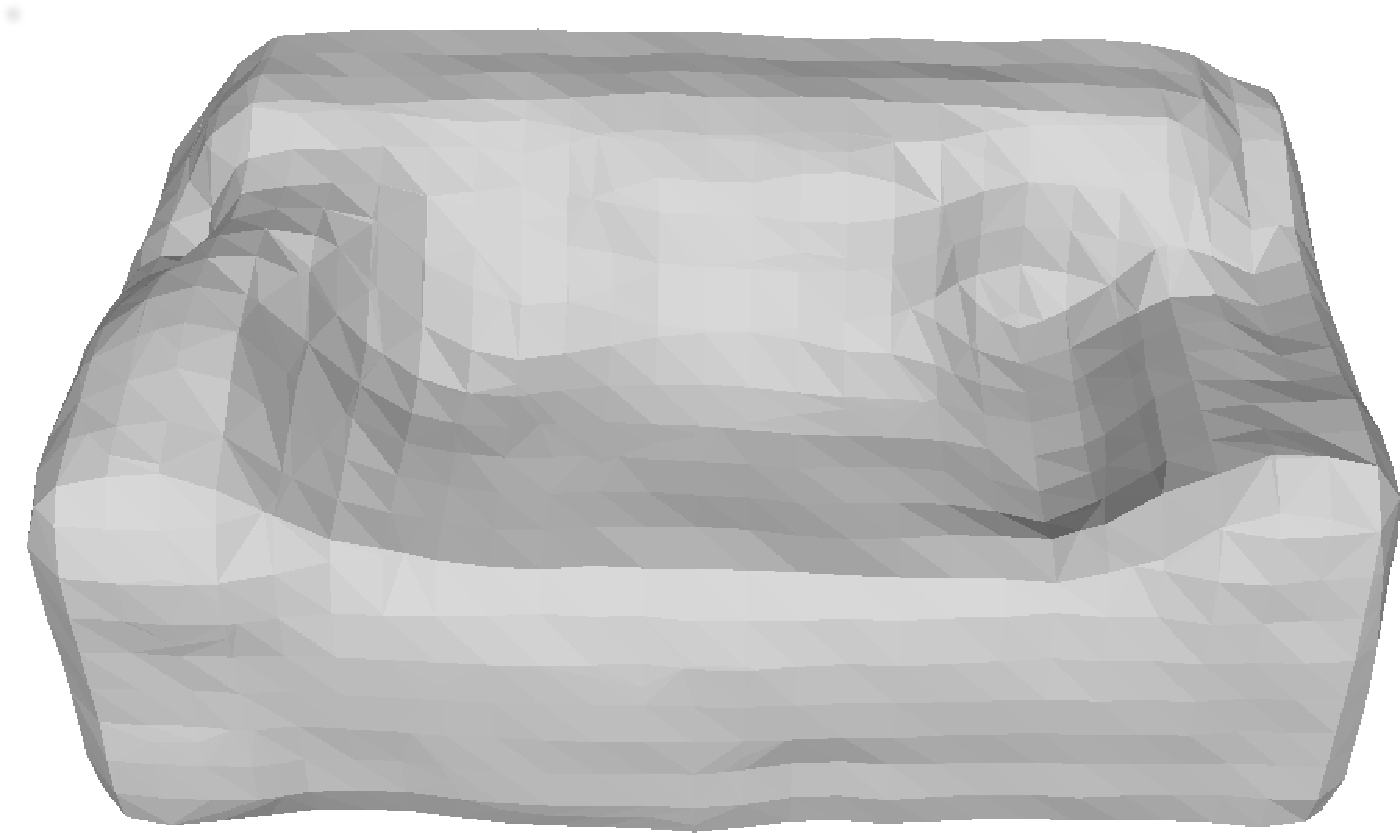
\includegraphics[width=0.8\linewidth]{images/epn-sofa1.pdf}
\end{subfigure}%

\vspace{0.1cm}
\begin{subfigure}[t]{0.19\linewidth}
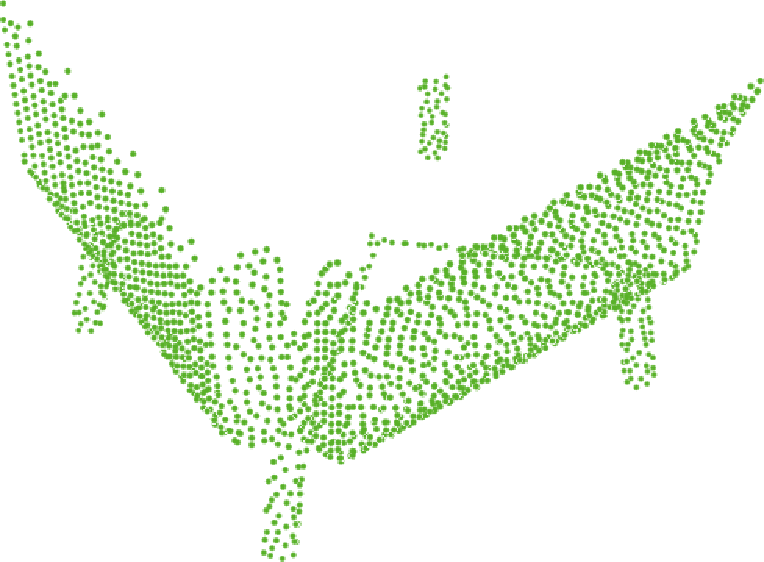
\includegraphics[width=0.9\linewidth]{images/pc-chair1.pdf}
\end{subfigure}
\hfill
\begin{subfigure}[t]{0.19\linewidth}
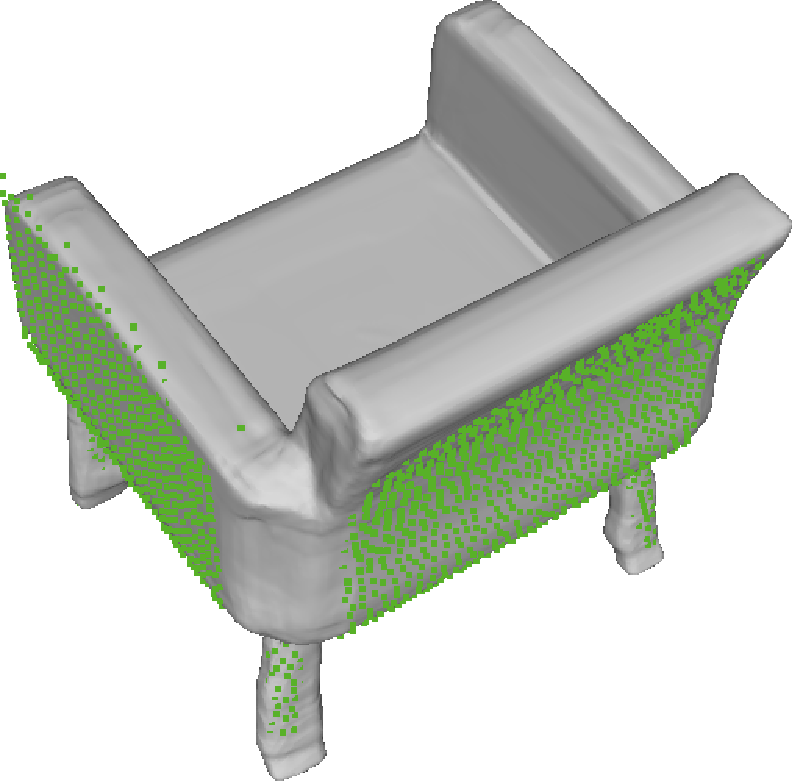
\includegraphics[width=0.9\linewidth]{images/overlay-chair1-1.pdf}
\end{subfigure}
\hfill
\begin{subfigure}[t]{0.16\linewidth}
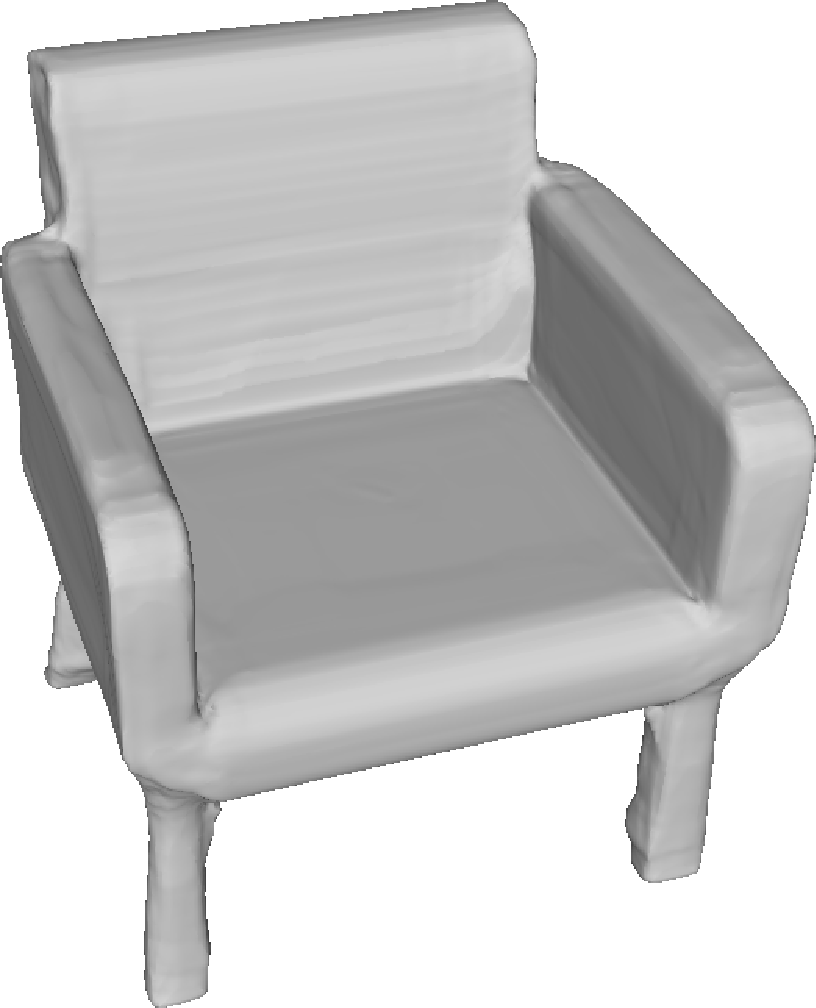
\includegraphics[width=0.9\linewidth]{images/secondview-chair-1.pdf}
\end{subfigure}
\hfill
\begin{subfigure}[t]{0.16\linewidth}
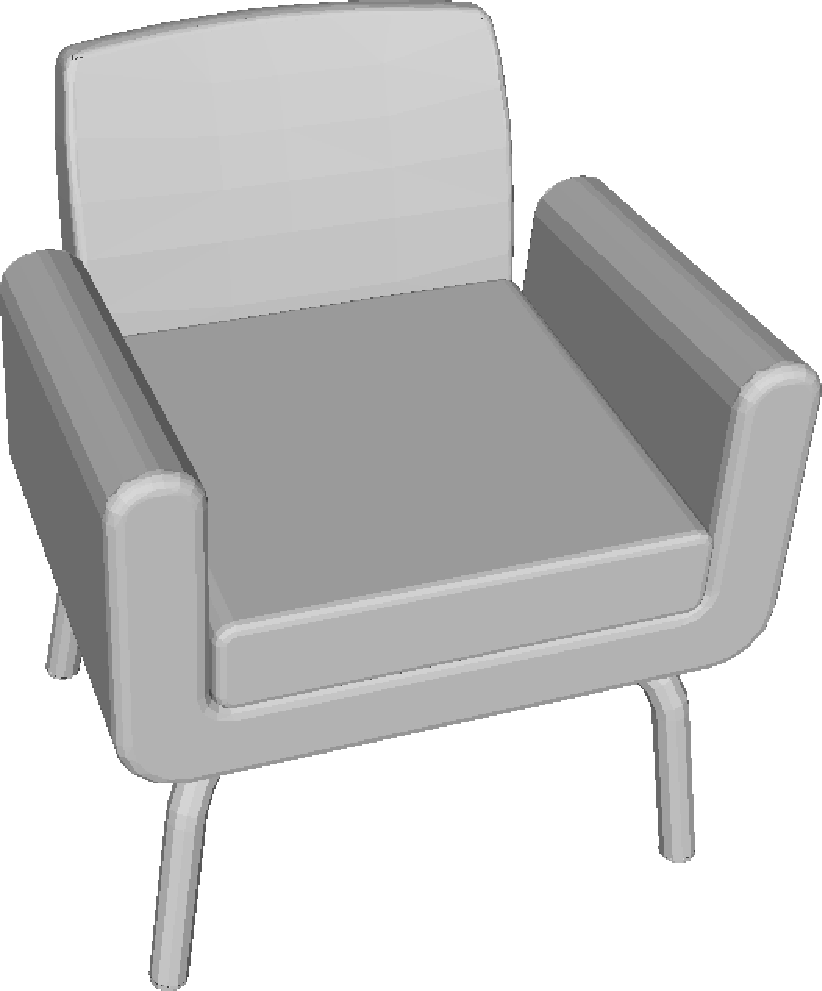
\includegraphics[width=0.9\linewidth]{images/gt-chair-1.pdf}
\end{subfigure}
\hfill
\begin{subfigure}[t]{0.14\linewidth}
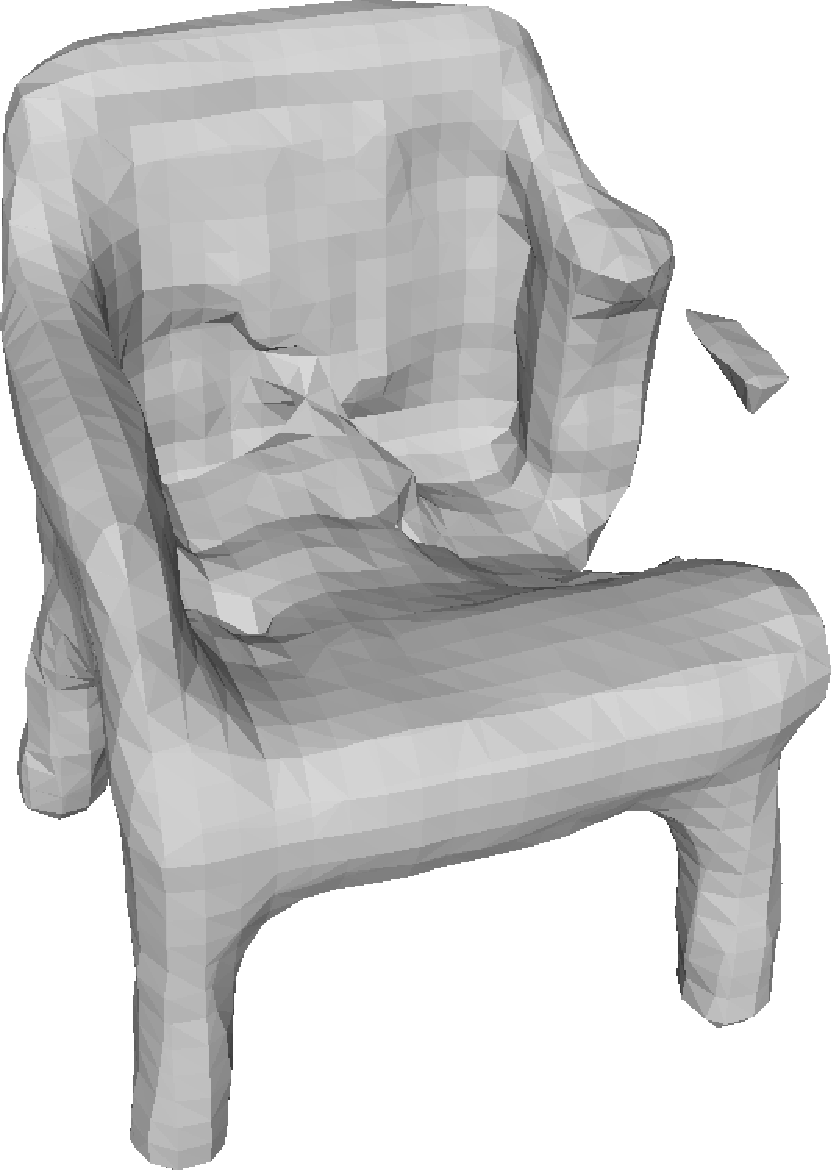
\includegraphics[width=0.9\linewidth]{images/chair-epn-1.pdf}
\end{subfigure}%

\begin{subfigure}[t]{0.21\linewidth}
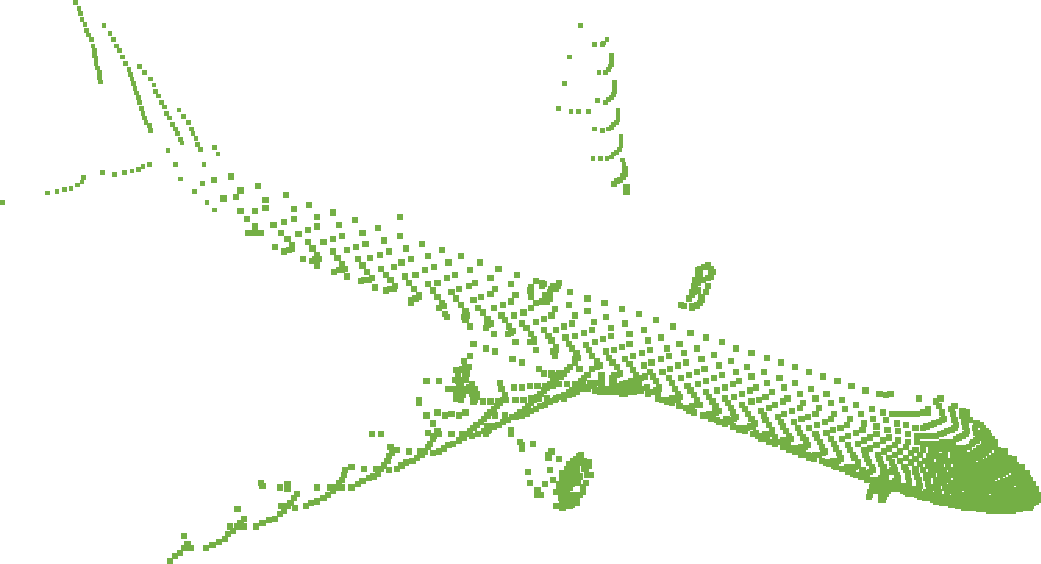
\includegraphics[width=0.9\linewidth]{images/plane-pc.pdf}
\caption{Input Depth}
\end{subfigure}
\hfill
\begin{subfigure}[t]{0.21\linewidth}
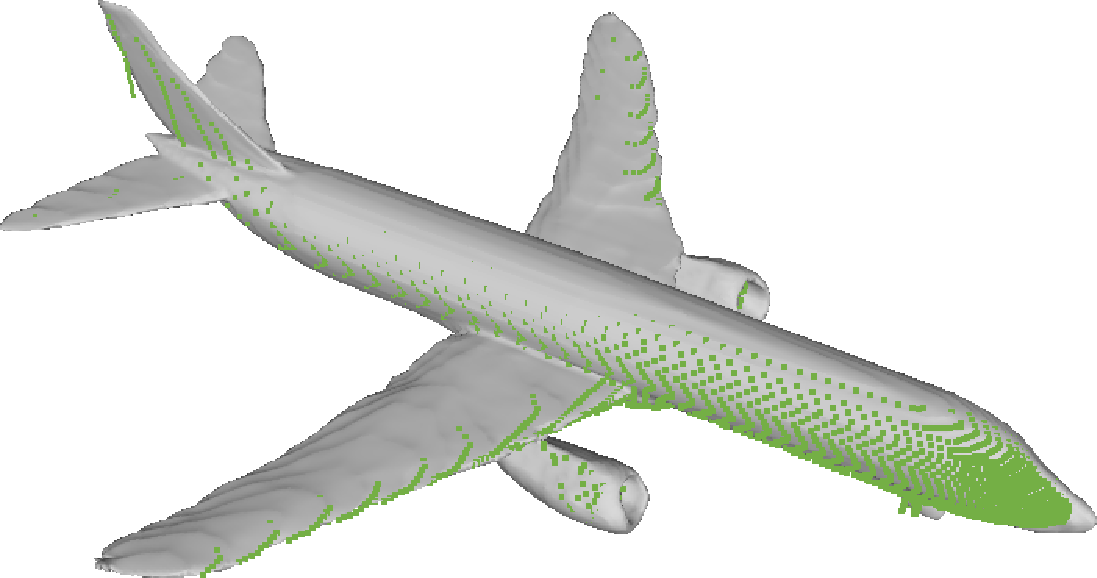
\includegraphics[width=0.9\linewidth]{images/overlay-plane.pdf}
\caption{Completion (ours)}
\end{subfigure}
\hfill
\begin{subfigure}[t]{0.18\linewidth}
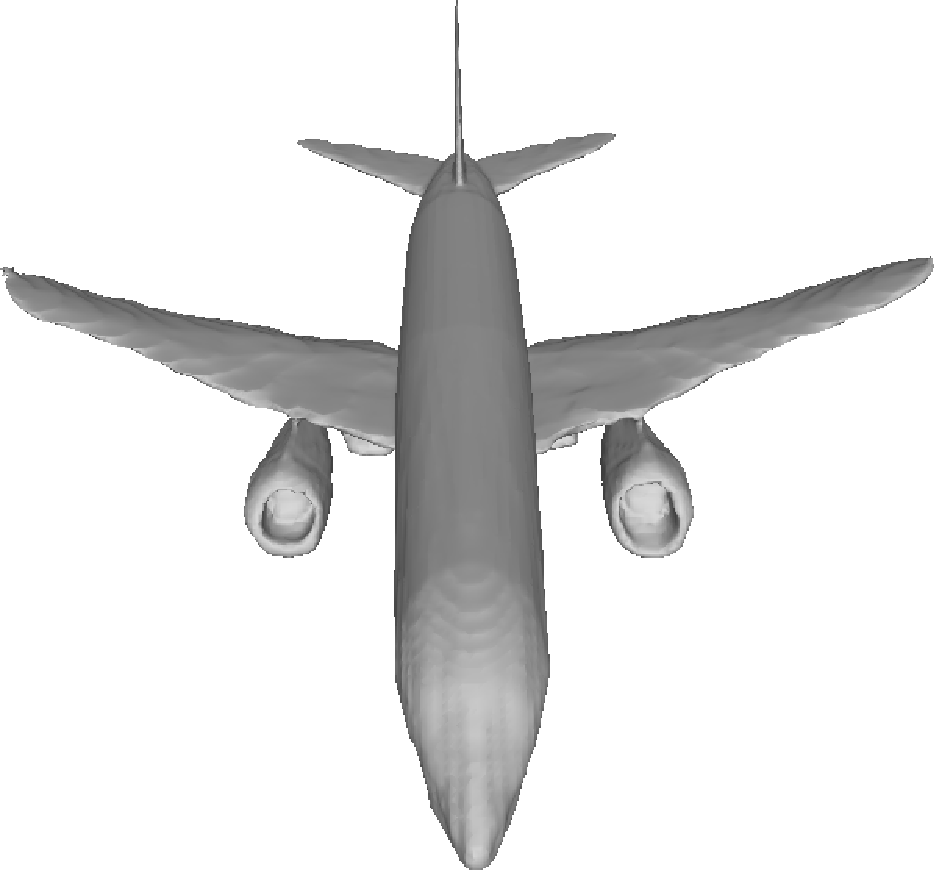
\includegraphics[width=0.9\linewidth]{images/completion-plane.pdf}
\caption{Second View (ours)}
\end{subfigure}
\hfill
\begin{subfigure}[t]{0.18\linewidth}
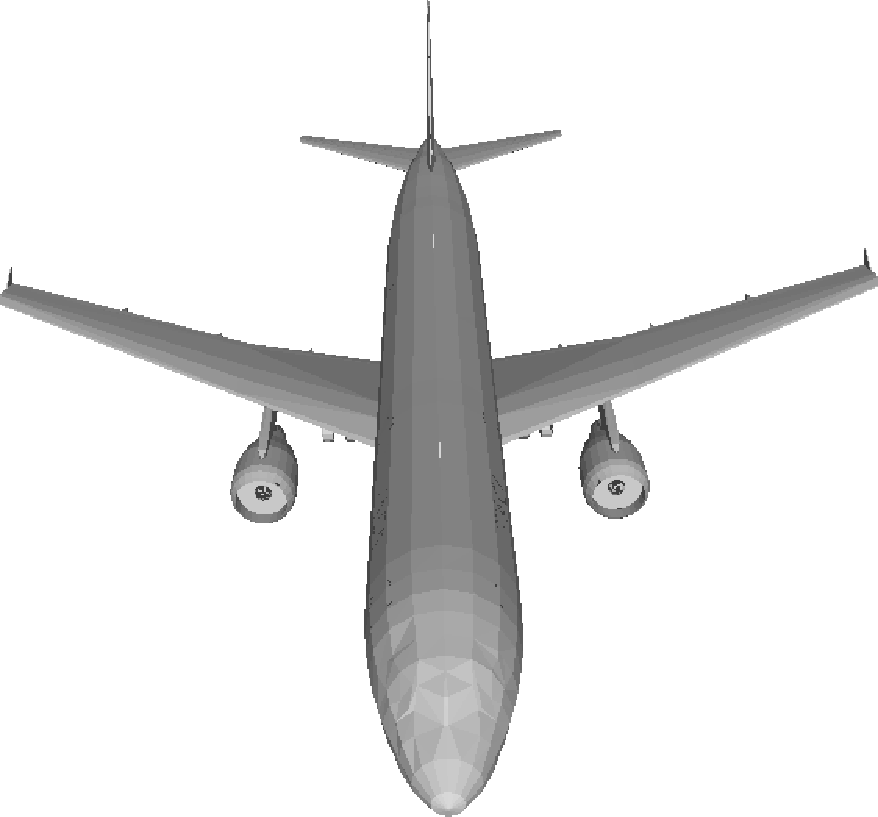
\includegraphics[width=0.9\linewidth]{images/gt-plane.pdf}
\caption{Ground truth}
\end{subfigure}
\hfill
\begin{subfigure}[t]{0.167\linewidth}
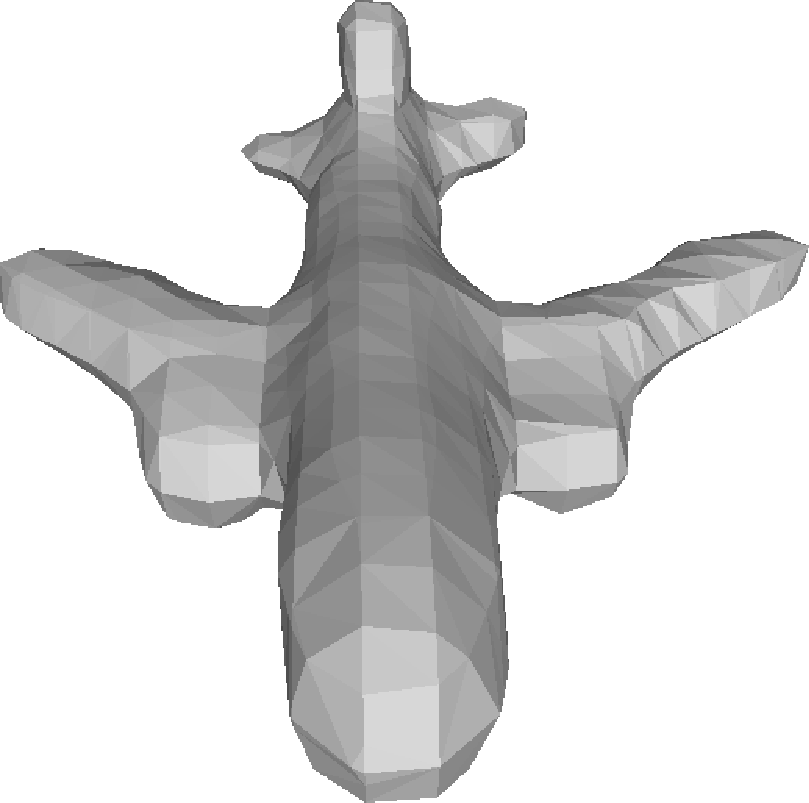
\includegraphics[width=0.9\linewidth]{images/epn-plane.pdf}
\caption{3D-EPN}
\end{subfigure}%
	\caption{For a given depth image visualized as a green point cloud, we show a comparison of shape completions from our DeepSDF approach against the true shape and 3D-EPN.}
	\label{fig: completion}
\end{figure*}

